\section{Обоснование актуальности}

На данный момент, практически отсутствуют системы, которые позволяют решать поставленную задачу. Для xUnit тестов можно построить стандартный отчет, но он подходит только для модульного тестирования, то есть в нем нет возможности сохранения дополнительной информации о ходе теста, сценария теста. Также у некоторых тестовых фремворков есть свои отчеты (например, Thucydides), но они узконаправленные, и позволяют действовать только в рамках соответсвующих фремворков. Для большинства членов семейства xUnit систем построения отчетов, кроме стандартного, нет.

Из-за отстутствия универсального решения, и наличия большого числа высокоуровневых тестов, анализ результатов отнимает очень много времени и сил. И часто узкое причина длинного цикла разработки именно затянувшийся процесс тестирования.

\section{Обзор существующих систем}

\subsection{Surefire}
Семейство xUnit предлагает стандартный отчет, который называется surefire. Это простой отчет, содержащий список тестов, и для каждого теста информацию о его статусе, времени работы и сообщения об ошибке (если имеется). Данное решение подходит для анализа результатов модульных тестов, но не годиться в рамках поставленной задачи.

\subsection{Thucydides}
Thucydides --- тестовый фремворк на основе jUnit. Он предоставляет возможность писать WebDriver'ные тесты, есть возможность разбивать тесты на шаги, и сохранять скриншоты. Основным недостатоком данной системы является то, что она слишком узконаправленная, и накладывает слишком много ограничений на как тесты и тестируемые системы. 

\section{Технический и организационный контекст}
Рассмотрим структуру разработки системы отчетов автотестов. Автор работы является основным разработчиком фремворка (Allure), активно взаимодействует с остальными участниками разработки. Основным заказчиком является отдел тестирования компании Яндекс, в лице Ерошенко Артема Михайловича, который также является основным идейным вдохновителем и руководителем разработки. 

Первый прототип, а так же первые две версии были спроектированы и разработаны автором данной работы, совмество с Артемом Михайловичем. Дальше к разработке присоеденился профессиональный front-end разработчик Сердюк Борис Дмитриевич, который переработал "морду" отчета, и до сих пор активно участвует в поддержке и развитии фреймворка. 

Изначально перед автором стояла задача предложить структуру фремворка, разработать прототип и адаптировать фремворк под работу с jUnit и pyTest. 

Общую схему работы фреймворка можно увидеть на рисунке \ref{fig:allure}.

\begin{figure}[htb]
\centering
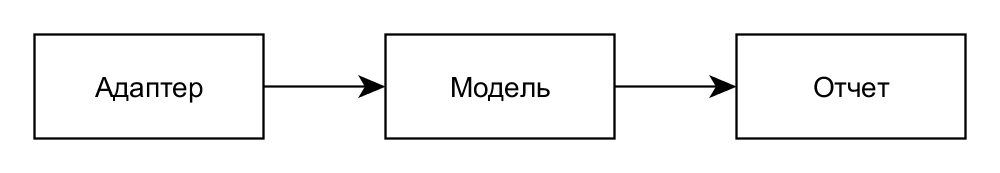
\includegraphics[height=30mm]{allure.png}
\caption{Общая схема работы Allure}
\label{fig:allure}
\end{figure}

Фактически, работа фремворка состоит из двух частей. Сначала надо собрать данные о ходе выполнения тестов, а затем сгенерировать из них отчет. 

\section{Уточненные требования к работе}

Обобщая вышесказанное, выведем следующие основные цели данной работы:

\begin{itemize}
\item разработать систему, позволяющую собирать дополнительную информацию о теста и отображать ее в виде отчета:
\begin{itemize}
\item система должна легко подключаться к большому числу уже написанных тестов;
\item система должна легко адаптироваться под разные языки программирования;
\item система должна быть модульной, легко расширяться;
\end{itemize}
\item написать первый прототип системы;
\item реализовать первую версию программы;
\item протестировать систему в реальных условиях;
\item проанализировать результаты работы системы.
\end{itemize}

Результатом данной работы будет являться готовый роботоспособный фремворк, активно используемый в тестировании в качестве универсального способа
отображения результатов работы автотестов.